\chapter{Adversarial Search}



\section{Section 1: Minimax Game-Playing Procedure (Q6.1)}

\subsection{1. Definition and Working Principle}
\textbf{Minimax} is a recursive decision-making algorithm used in two-player, zero-sum, perfect-information games (e.g., Chess, Tic-Tac-Toe). 
\begin{itemize}
  \item   \textbf{Zero-sum:} The utility gained by one player is exactly equal to the utility lost by the opponent.
  \item   \textbf{Two Players:}
  \item   \textbf{MAX:} Tries to maximize the final utility score.
  \item   \textbf{MIN:} Tries to minimize MAX's final utility score (maximizing their own advantage).
\end{itemize}

The algorithm performs a depth-first search of the game tree. It computes the utility values of leaf nodes and propagates them upward:
\textit{   At a \textbf{MAX node}, the value is the }maximum* of the children's values.
\textit{   At a \textbf{MIN node}, the value is the }minimum* of the children's values.

\begin{figure}[H]
\centering
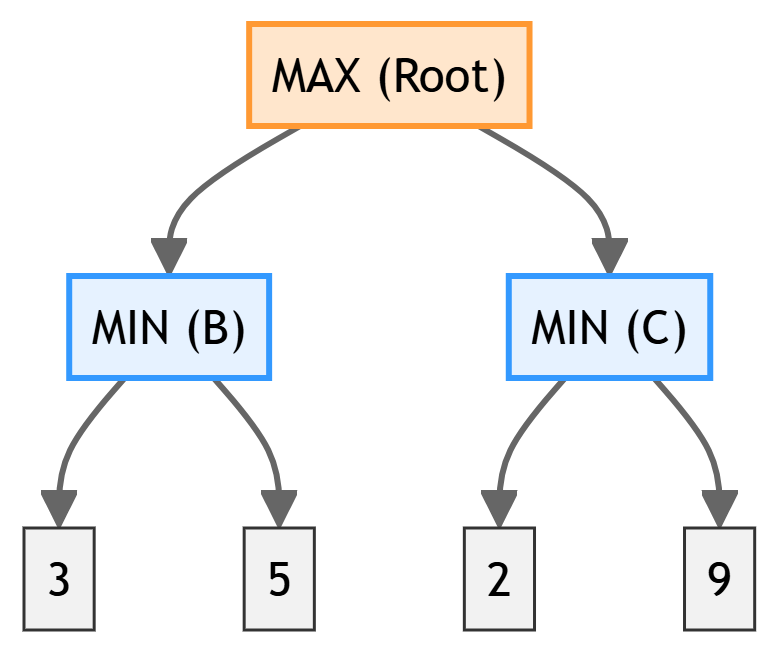
\includegraphics[width=0.75\textwidth,height=0.32\textheight,keepaspectratio]{../Images/chapter_06/minimax_tree.png}
\caption{Minimax Game Tree}
\end{figure}

\subsection{2. Time and Space Complexity}
\begin{itemize}
  \item   \textbf{Time Complexity:} $O(b^d)$, where $b$ is the branching factor (legal moves) and $d$ is the maximum depth of the game tree.
  \item   \textbf{Space Complexity:} $O(bd)$ (Linear space, similar to DFS, storing the active path from root to leaf).
\end{itemize}


\section{Section 2: Alpha-Beta Pruning (Q6.2)}

\subsection{1. Working Principle}
\textbf{Alpha-Beta Pruning} is an optimization technique for the minimax algorithm that cuts off branches that cannot possibly influence the final decision. It maintains two values throughout the search:
\begin{itemize}
  \item   \textbf{Alpha ($\alpha$):} The value of the best (highest-value) choice found so far at any choice point along the path for MAX. Initialized to $-\infty$.
  \item   \textbf{Beta ($\beta$):} The value of the best (lowest-value) choice found so far at any choice point along the path for MIN. Initialized to $+\infty$.
\end{itemize}

\subsubsection{The Pruning Rule:}
During search, if a node's beta value is less than or equal to its alpha value ($\beta \le \alpha$), the remaining children of that node do not need to be evaluated (they are pruned).

\begin{itemize}
  \item   \textbf{Alpha-Cutoff ($\alpha$-cutoff):} Occurs at a MIN node when it discovers a value less than or equal to the alpha value of a parent MAX node.
  \item   \textbf{Beta-Cutoff ($\beta$-cutoff):} Occurs at a MAX node when it discovers a value greater than or equal to the beta value of a parent MIN node.
\end{itemize}


\subsection{2. Trace Example: 3-Level Branching Game Tree}

Let's execute Minimax and Alpha-Beta Pruning on the game tree shown in Figure 1, where \textbf{MAX} is at the root node (A), \textbf{MIN} is at level 1 (B, C, D), and MAX is at level 2 (E to K).

\begin{figure}[H]
\centering
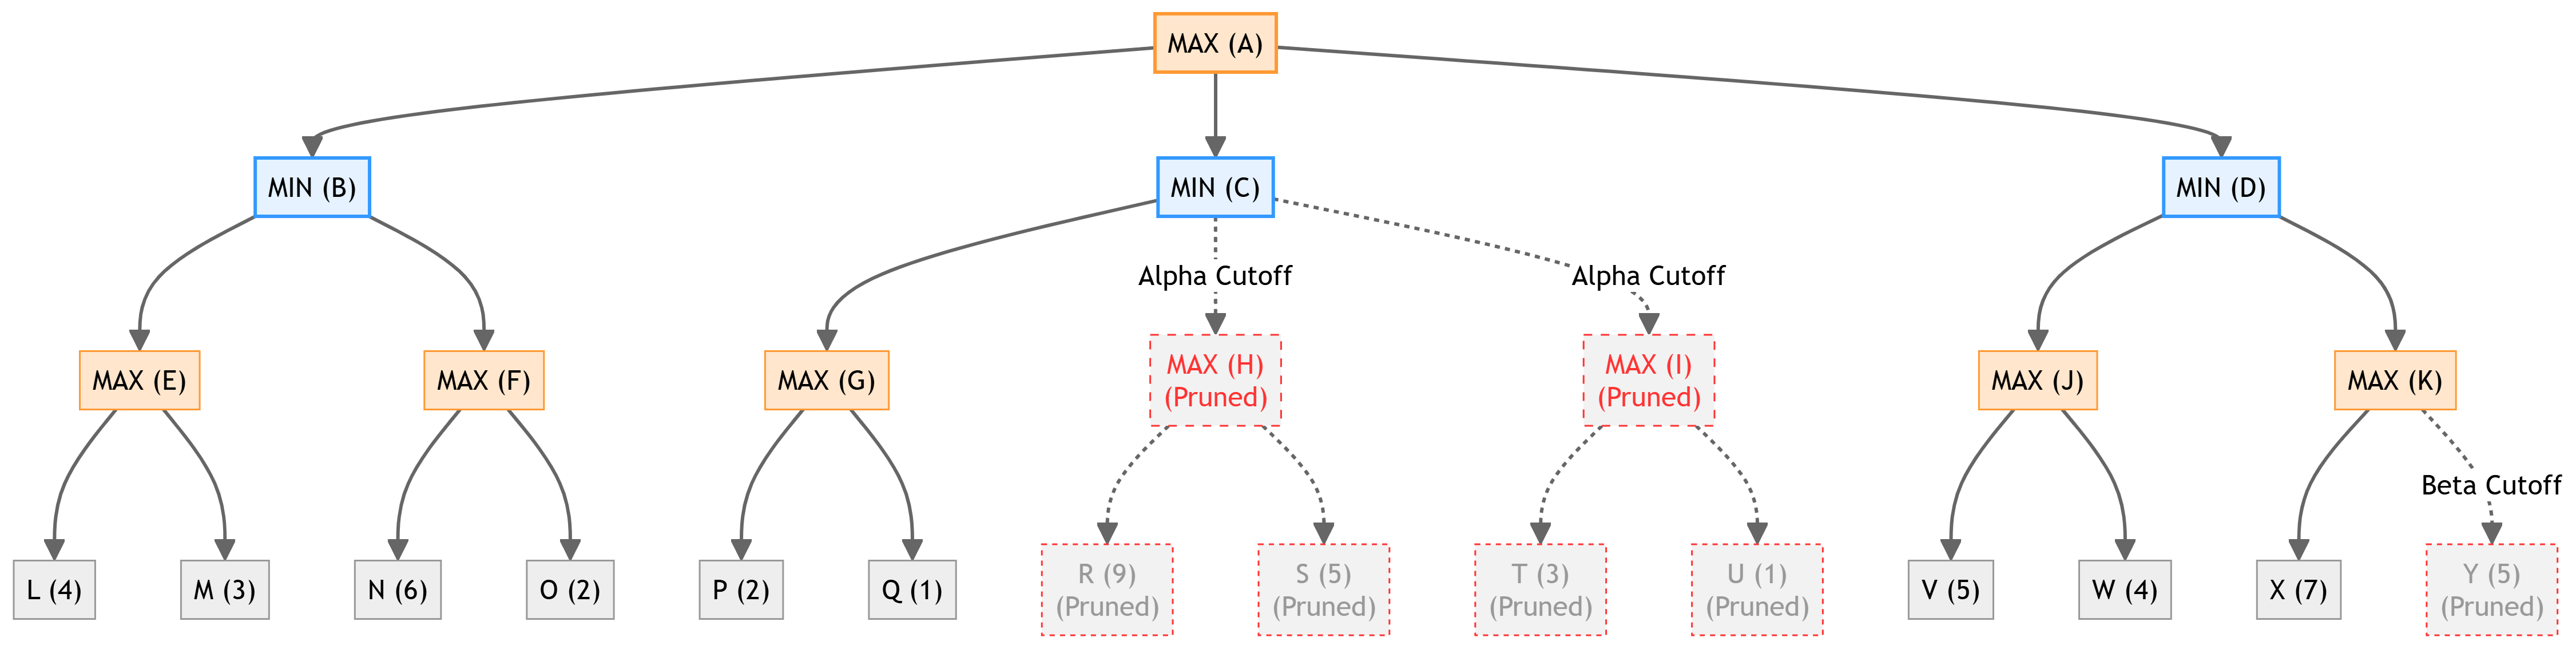
\includegraphics[width=0.75\textwidth,height=0.32\textheight,keepaspectratio]{../Images/chapter_06/alphabeta_tree.png}
\caption{Alpha-Beta Pruning Game Tree}
\end{figure}

\subsubsection{Step-by-Step Pruning and Minimax Trace:}

\#\#\#\#\# \textbf{Branch B (Left Side of Root):}
\begin{enumerate}
  \item \textbf{Analyze Node E:}
\end{enumerate}
\begin{itemize}
  \item   Children: L ($4$) and M ($3$).
  \item   Since E is a MAX node, $Value(E) = \max(4, 3) = 4$.
  \item   Propagate to B: Since B is a MIN node, B's current beta ($\beta_B$) becomes $\min(+\infty, 4) = 4$.
\end{itemize}
\begin{enumerate}
  \item \textbf{Analyze Node F:}
\end{enumerate}
\begin{itemize}
  \item   Children: N ($6$) and O ($2$).
  \item   Since F is a MAX node, $Value(F) = \max(6, 2) = 6$.
  \item   Propagate to B: $\beta_B = \min(4, 6) = 4$.
\end{itemize}
\begin{enumerate}
  \item \textbf{Evaluate Node B:}
\end{enumerate}
\begin{itemize}
  \item   Since E ($4$) and F ($6$) are evaluated, $Value(B) = \min(4, 6) = 4$.
  \item   Propagate to Root A: Since A is a MAX node, A's alpha ($\alpha_A$) becomes $\max(-\infty, 4) = 4$.
\end{itemize}


\#\#\#\#\# \textbf{Branch C (Middle of Root):}
We search with $\alpha = 4$ and $\beta = +\infty$.
\begin{enumerate}
  \item \textbf{Analyze Node G:}
\end{enumerate}
\begin{itemize}
  \item   Children: P ($2$) and Q ($1$).
  \item   Since G is a MAX node, $Value(G) = \max(2, 1) = 2$.
  \item   Propagate to C (MIN node): $\beta_C$ becomes $\min(+\infty, 2) = 2$.
  \item   \textbf{Check Pruning Condition at C:}
  \item   We have $\alpha_C = 4$ (passed down from A) and $\beta_C = 2$.
  \item   Since $\beta_C \le \alpha_C$ ($2 \le 4$), an \textbf{Alpha-Cutoff} occurs at MIN node C!
  \item   The remaining children of C (nodes \textbf{H} and \textbf{I}) are \textbf{pruned}.
  \item   Thus, we do not examine leaves \textbf{R ($9$), S ($5$), T ($3$), U ($1$)}.
  \item   $Value(C) = 2$.
\end{itemize}


\#\#\#\#\# \textbf{Branch D (Right Side of Root):}
We search with $\alpha = 4$ and $\beta = +\infty$.
\begin{enumerate}
  \item \textbf{Analyze Node J:}
\end{enumerate}
\begin{itemize}
  \item   Children: V ($5$) and W ($4$).
  \item   Since J is a MAX node, $Value(J) = \max(5, 4) = 5$.
  \item   Propagate to D (MIN node): $\beta_D$ becomes $\min(+\infty, 5) = 5$.
  \item   At this point, $\alpha_D = 4$ and $\beta_D = 5$. (No pruning yet).
\end{itemize}
\begin{enumerate}
  \item \textbf{Analyze Node K:}
\end{enumerate}
\begin{itemize}
  \item   Children: X ($7$).
  \item   \textbf{Check Pruning Condition at K:}
  \item   K is a MAX node, currently evaluating child X ($7$).
  \item   $Value(K) \ge 7$.
  \item   Since D is a MIN node above K, D's beta $\beta_D = 5$.
  \item   If K's value is $\ge 7$, D (MIN) will definitely choose J ($5$) over K ($\ge 7$).
  \item   Therefore, since $Value(K) \ge 7 > \beta_D$ ($7 \ge 5$), a \textbf{Beta-Cutoff} occurs at MAX node K!
  \item   The remaining child of K (node \textbf{Y ($5$)}) is \textbf{pruned}.
\end{itemize}
\begin{enumerate}
  \item \textbf{Evaluate Node D:}
\end{enumerate}
\begin{itemize}
  \item   $Value(D) = \min(Value(J), Value(K)) = \min(5, 7) = 5$.
\end{itemize}


\#\#\#\#\# \textbf{Evaluate Root A:}
\begin{itemize}
  \item   $Value(A) = \max(Value(B), Value(C), Value(D)) = \max(4, 2, 5) = 5$.
  \item   \textbf{Optimal Move for Maximizer:} Choose move to \textbf{Node D}.
\end{itemize}

\subsubsection{Final Audit Summary:}
\begin{itemize}
  \item   \textbf{Minimax values of intermediate nodes:}
  \item   $E = 4$, $F = 6$, $G = 2$, $J = 5$, $K = 7$.
  \item   $B = 4$, $C = 2$, $D = 5$, $A = 5$.
  \item   \textbf{Pruned Branches:}
  \item   Nodes \textbf{H} and \textbf{I} (and their children R, S, T, U) via \textbf{Alpha-Cutoff} at node C.
  \item   Leaf \textbf{Y} via \textbf{Beta-Cutoff} at node K.
  \item   \textbf{Number of terminal leaves examined:} $9$ out of $14$ leaves (L, M, N, O, P, Q, V, W, X).
\end{itemize}
